\usetikzlibrary{arrows.meta,fit,matrix,patterns}

\tikzset{
    stackBox/.style={very thick},
    allocBox/.style={dashed,very thick,fill=blue!20},
    onStack/.style={thick},
    frameOne/.style={fill=blue!15},
    frameTwo/.style={fill=red!15},
    markLine/.style={blue!50!black},
    markLineB/.style={red!90!black},
    hiLine/.style={red!90!black},
}
\begin{frame}<1-6>[fragile,label=lkpTble]{allocations and lookup table}
    \begin{tikzpicture}
        \draw[onStack] (0, 0) rectangle (4, -7);
        \draw[allocBox] (0, 0) rectangle (4, -0.4);
        \draw[stackBox] (0, 0) rectangle (4, -0.5);
        \draw[allocBox] (0, -0.5) rectangle (4, -0.8);
        \draw[stackBox] (0, -0.5) rectangle (4, -1.0);
        \draw[allocBox] (0, -1) rectangle (4, -1.9);
        \draw[stackBox] (0, -1) rectangle (4, -2);
        \draw[allocBox] (0, -2) rectangle (4, -2.4);
        \draw[stackBox] (0, -2) rectangle (4, -2.5);
        \draw[allocBox] (0, -2.5) rectangle (4, -2.7);
        \draw[stackBox] (0, -2.5) rectangle (4, -3);
        \draw[stackBox] (0, -3) rectangle (4, -4);
        \draw[allocBox] (0, -4) rectangle (4, -5.2);
        \draw[stackBox] (0, -4) rectangle (4, -6);

        \begin{visibleenv}<1->
            \node[anchor=north west,align=left] at (9, 0) {
                object allocated in \\ \myemph<1>{power-of-two `slots'}
            };
        \end{visibleenv}
        \begin{visibleenv}<2->
            \matrix[tight matrix,
                nodes={text width=1cm,font=\small\tt},anchor=north west,label={north:table}] (tbl) at (7, -1) {
                $2^4$ \\ $2^4$  \\ $2^5$ \\ $2^5$ \\ $2^4$ \\ $2^4$ \\
                $0$ \\ $0$ \\
                $2^6$ \\ $2^6$ \\ $2^6$ \\ $2^6$ \\
            };
            \begin{scope}[thick,dotted,-Latex]
            \draw (4, -.25) -- (tbl-1-1.west);
            \draw (4, -.75) -- (tbl-2-1.west);
            \draw (4, -1.25) -- (tbl-3-1.west);
            \draw (4, -1.75) -- (tbl-4-1.west);
            \draw (4, -2.25) -- (tbl-5-1.west);
            \draw (4, -2.75) -- (tbl-6-1.west);
            \draw (4, -3.25) -- (tbl-7-1.west);
            \draw (4, -3.75) -- (tbl-8-1.west);
            \draw (4, -4.25) -- (tbl-9-1.west);
            \end{scope}
        \end{visibleenv}
        \begin{visibleenv}<3>
            \draw[ultra thick,red] (0, -1) rectangle (4, -2);
            \node[draw,ultra thick,red,inner sep=0mm,fit=(tbl-3-1) (tbl-4-1)] {};
            \draw[ultra thick,blue] (0, -4) rectangle (4, -6);
            \node[draw,ultra thick,blue,inner sep=0mm,fit=(tbl-9-1) (tbl-12-1)] {};
        \end{visibleenv}
        \begin{visibleenv}<3->
            \node[anchor=north west,align=left] at (9, -2) {
                table stores sizes \\
                \myemph{for each 16 bytes}
            };
        \end{visibleenv}
        \begin{visibleenv}<4>
            \draw[ultra thick,red] (0, -3) rectangle (4, -4);
            \node[draw,ultra thick,red,inner sep=0mm,fit=(tbl-7-1) (tbl-8-1)] {};
        \end{visibleenv}
        \begin{visibleenv}<4->
            \node[anchor=north west,align=left] at (9, -3.5) {
                addresses \textbf<4>{multiples of size} \\
                (may \myemph{require padding})
            };
        \end{visibleenv}
        \begin{pgfonlayer}{bg}
        \begin{visibleenv}<5>
            \fill[red!30] (0, -5.2) rectangle (4, -6.);
            \fill[red!30] (0, -2.7) rectangle (4, -3.);
            \fill[red!30] (0, -1.9) rectangle (4, -2.);
            \fill[red!30] (0, -2.4) rectangle (4, -2.5);
            \fill[red!30] (0, -0.8) rectangle (4, -1.);
            \fill[red!30] (0, -0.4) rectangle (4, -0.5);
        \end{visibleenv}
        \end{pgfonlayer}
        \begin{visibleenv}<5->
            \node[anchor=north west,align=left] at (9, -5.5) {
                sizes are \textbf<5>{powers of two} \\
                (may \myemph{require padding})
            };
        \end{visibleenv}
    \end{tikzpicture}
\end{frame}

\begin{frame}[fragile,label=managing]{managing the table}
    \begin{itemize}
        \item not just done \texttt{malloc()/new}
        \item also for stack allocations:
    \end{itemize}
    \begin{lstlisting}[style=small,language=C]
void vulnerable() {
    char buffer[100];
    gets(vulnerable);
}
\end{lstlisting}
    \begin{tikzpicture}[remember picture, overlay]
        \node[anchor=north east] at ([xshift=-.25cm, yshift=-1cm]current page.north east) {
    \begin{lstlisting}[style=small,language=myasm]
vulnerable:
  // make %rsp a multiple
  // of 128 (2^7) 
  andq $0xFFFFFFFFFFFFFF80, %rsp
  // allocate 128 bytes
  subq $0x80, %rsp
  // rax <- rsp / 16
  movq $rsp, %rax
  shrq $4, %rax
  movb $7, TABLE(%rax)
  movb $7, TABLE+1(%rax)
  ...
  movq %rsp, %rdi
  call gets
  ret
\end{lstlisting}
};
    \end{tikzpicture}
\end{frame}

\begin{frame}[fragile,label=sparseLookup]{sparse lookup table}
    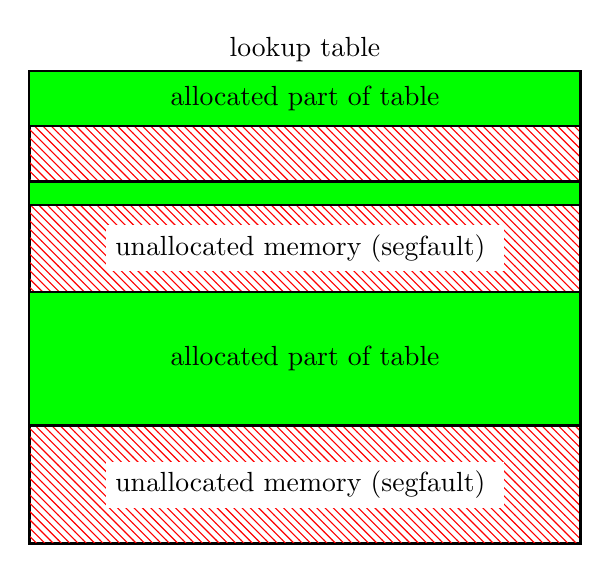
\begin{tikzpicture}
        \node[anchor=south] at (3.5, 3) {lookup table};
        \draw[stackBox] (0, 3) rectangle (7, -3);
        \draw[pattern color=red,pattern=north west lines,onStack] (0, -3) rectangle (7, -1.5)
            node[midway,fill=white,align=center] {unallocated memory (segfault) };
        \draw[fill=green,onStack] (0, -1.5) rectangle (7, .2)
            node[midway] { allocated part of table };
        \draw[pattern color=red,pattern=north west lines,onStack] (0, .20) rectangle (7, 1.3)
            node[midway,fill=white,align=center] {unallocated memory (segfault) };
        \draw[fill=green,onStack] (0, 1.3) rectangle (7, 1.6);
        \draw[pattern color=red,pattern=north west lines,onStack] (0, 1.6) rectangle (7, 2.3);
        \draw[fill=green,onStack] (0, 2.3) rectangle (7, 3)
            node[midway] { allocated part of table };
    \end{tikzpicture}
\end{frame}

